\documentclass[conference]{IEEEtran}
\IEEEoverridecommandlockouts
% The preceding line is only needed to identify funding in the first footnote. If that is unneeded, please comment it out.
\usepackage{cite}
\usepackage{amsmath,amssymb,amsfonts}
\usepackage{algorithmic}
\usepackage{graphicx}
\usepackage{textcomp}
\usepackage{xcolor}
\usepackage{graphicx}
\def\BibTeX{{\rm B\kern-.05em{\sc i\kern-.025em b}\kern-.08em
    T\kern-.1667em\lower.7ex\hbox{E}\kern-.125emX}}
\begin{document}

\title{Untersuchung der Nachweisbarkeit des Akkomodation-Vergenzkonflikts in einem EEG in einer VR entspannungs Szene\\
\thanks{HFU Furtwangen}
}

\author{
	\IEEEauthorblockN{Nick Philipp Häcker}
	\IEEEauthorblockA{\textit{Fakultät Digitale Medien} \\
	\textit{Hochschule Furtwangen}\\
	Furtwangen, Deutschland \\
	haeckern@hs-furtwangen.de}
	
	\and
	\IEEEauthorblockN{Suzan Johannes}
	\IEEEauthorblockA{\textit{Fakultät Digitale Medien} \\
	\textit{Hochschule Furtwangen}\\
	Furtwangen, Deutschland \\
	nick.philipp.haecker@hs-furtwangen.de}
	\and
	
	\IEEEauthorblockN{Patrick Kaserer}
	\IEEEauthorblockA{\textit{Fakultät Digitale Medien} \\
	\textit{Hochschule Furtwangen}\\
	Furtwangen, Deutschland \\
	patrick.kaserer@hs-furtwangen.de}
	\and
	
	\IEEEauthorblockN{Johann Schulenburg}
	\IEEEauthorblockA{\textit{Fakultät Digitale Medien} \\
	\textit{Hochschule Furtwangen}\\
	Furtwangen, Deutschland \\
	johann.schulenburg@hs-furtwangen.de}
	
	\and
	\IEEEauthorblockN{Lukas Willmann}
	\IEEEauthorblockA{\textit{Fakultät Digitale Medien} \\
	\textit{Hochschule Furtwangen}\\
	Furtwangen, Deutschland \\
	Lukas.willmann@hs-furtwangen.de}
}

\maketitle

\begin{abstract}
This document is a model and instructions for \LaTeX.
This and the IEEEtran.cls file define the components of your paper [title, text, heads, etc.]. *CRITICAL: Do Not Use Symbols, Special Characters, Footnotes, 
or Math in Paper Title or Abstract.
\end{abstract}

\begin{IEEEkeywords}
virtual reality, akkommodation-vergenz konflikt, elektroenzephalografie
\end{IEEEkeywords}

\section{Einleitung}
“Applications of Computer Science, including digital games, virtual reality, and augmented reality [...], have enormous potential for bringing about cultural change.” \cite{b3} Laut einer Prognose von ARtillery Intelligence soll zwischen 2021 bis 2026 der Umsatz von Virtual Reality weltweit von 8,3 auf 28,84 Milliarden US-Dollar steigen. \cite{b2} 
VR Brillen verwenden Stereoskopie, bei welcher jedem Auge leicht unterschiedliche Informationen durch eine horizontale Verschiebung der Bilder zugespielt werden, damit bei dem Nutzer eine 3D Wirkung der Darstellung entsteht. Durch die entstehenden Parallaxen kann die Szene den Eindruck erwecken, aus der Leinwand hervor zu stechen oder dahinter zu liegen.
Die hier beschriebene Untersuchung konzentriert sich auf den Accommodation Vergenz Konflikt. Dieser tritt gerade in der modernen VR Technologie auf, da durch die Linsen der VR Brille die Bildebene in eine weite Entfernung projiziert wird und die Objekte in VR durch die Interaktion in greifbarer Nähe sind.
“In order to see one object, the eyeballs need to rotate accordingly. This mechanism is called the “vergence”. In a natural situation, as an object is moving closer or further, vergence matches another physiological phenomena: “accommodation”. It enables the object’s image to remain clear on the retina. It is caused by a deformation of the crystalline lens, which focuses light beams the same way camera lenses do.”
Durch den Versuch soll aufgezeigt werden, ob mögliche Probleme in Anwendungen, welche in dem kritischen Bereich des Akkomodation-Vergenz Konflikt arbeiten, durch das EEG nachweisbar sind oder nicht. Somit kann sich zukünftige Forschung ebenfalls diesem Bereich widmen.

\section{Related Work}

\section{Methodik}

\section{Ergebnisse}

\begin{figure}[h!]
	\centering
	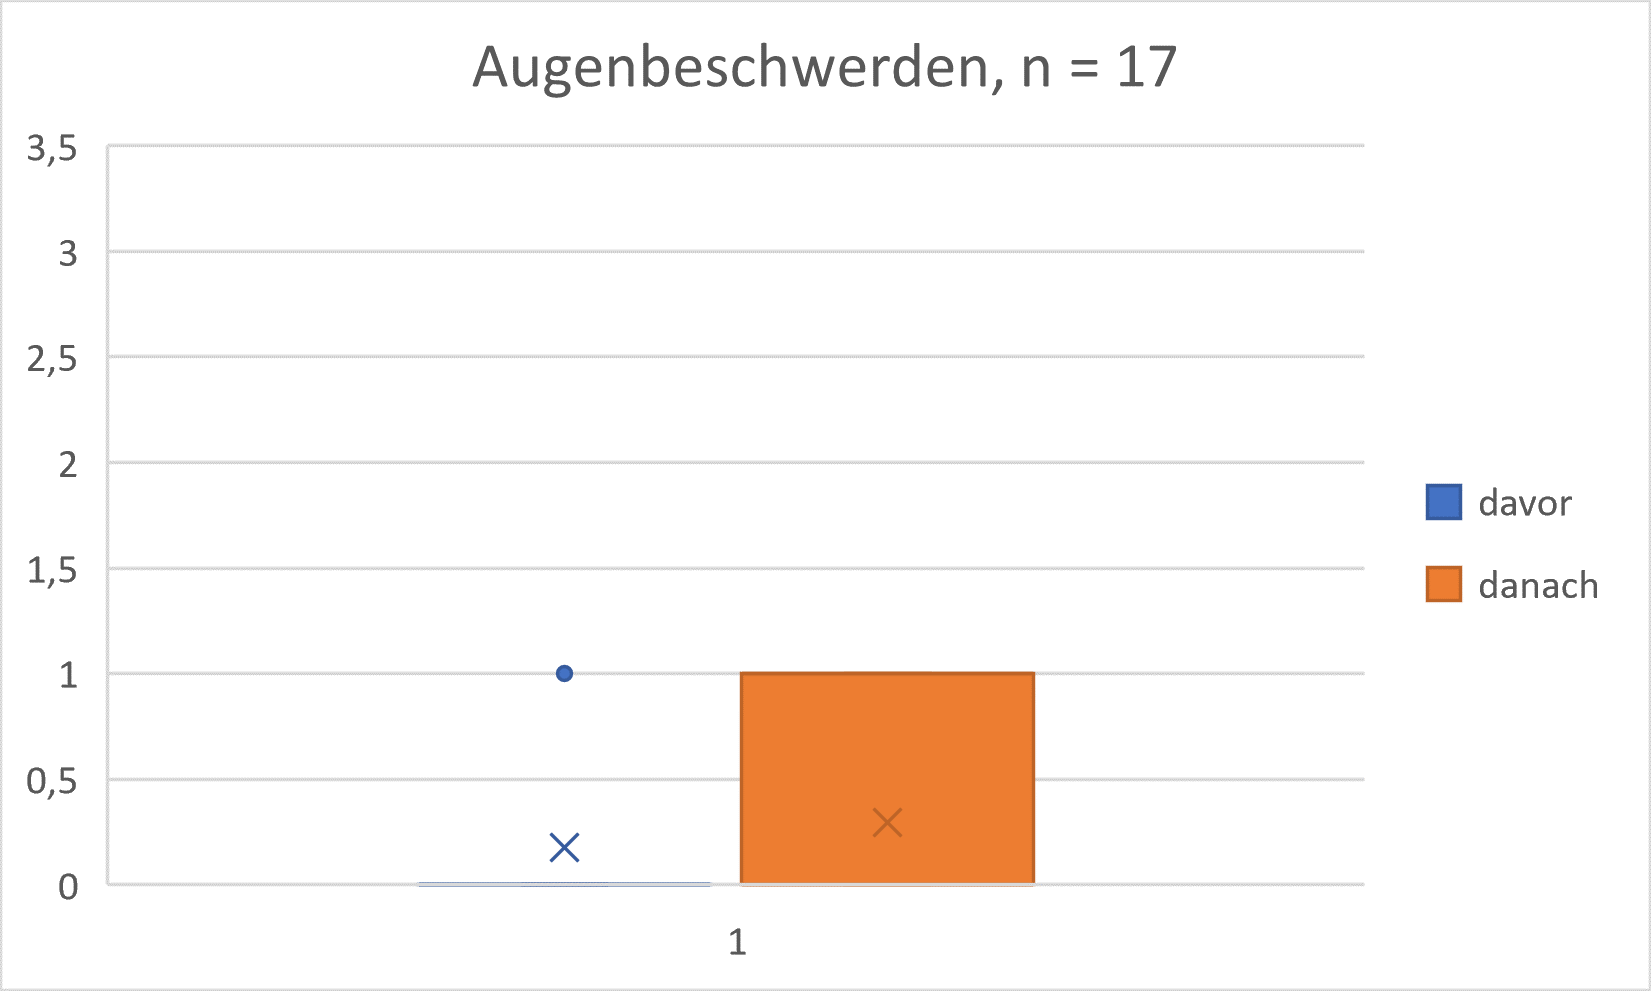
\includegraphics[width=0.2\textwidth]{assets/augenBesch.png} \hspace{-5pt}
	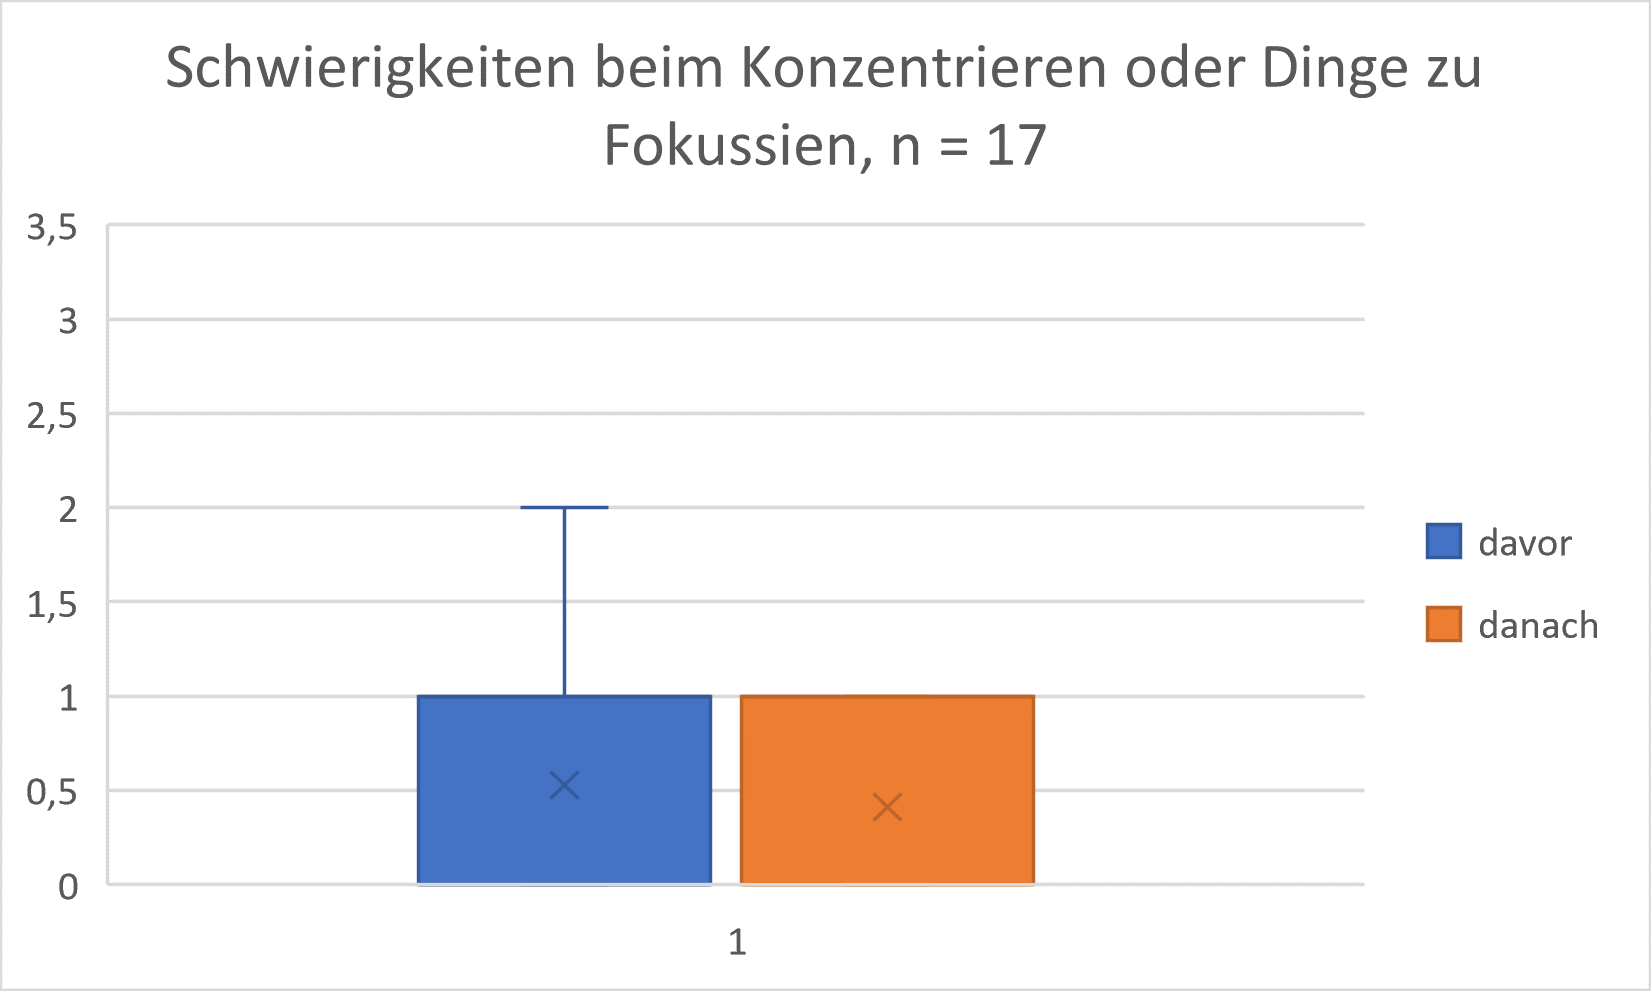
\includegraphics[width=0.2\textwidth]{assets/fokus.png} \\
	\vspace{2pt}
	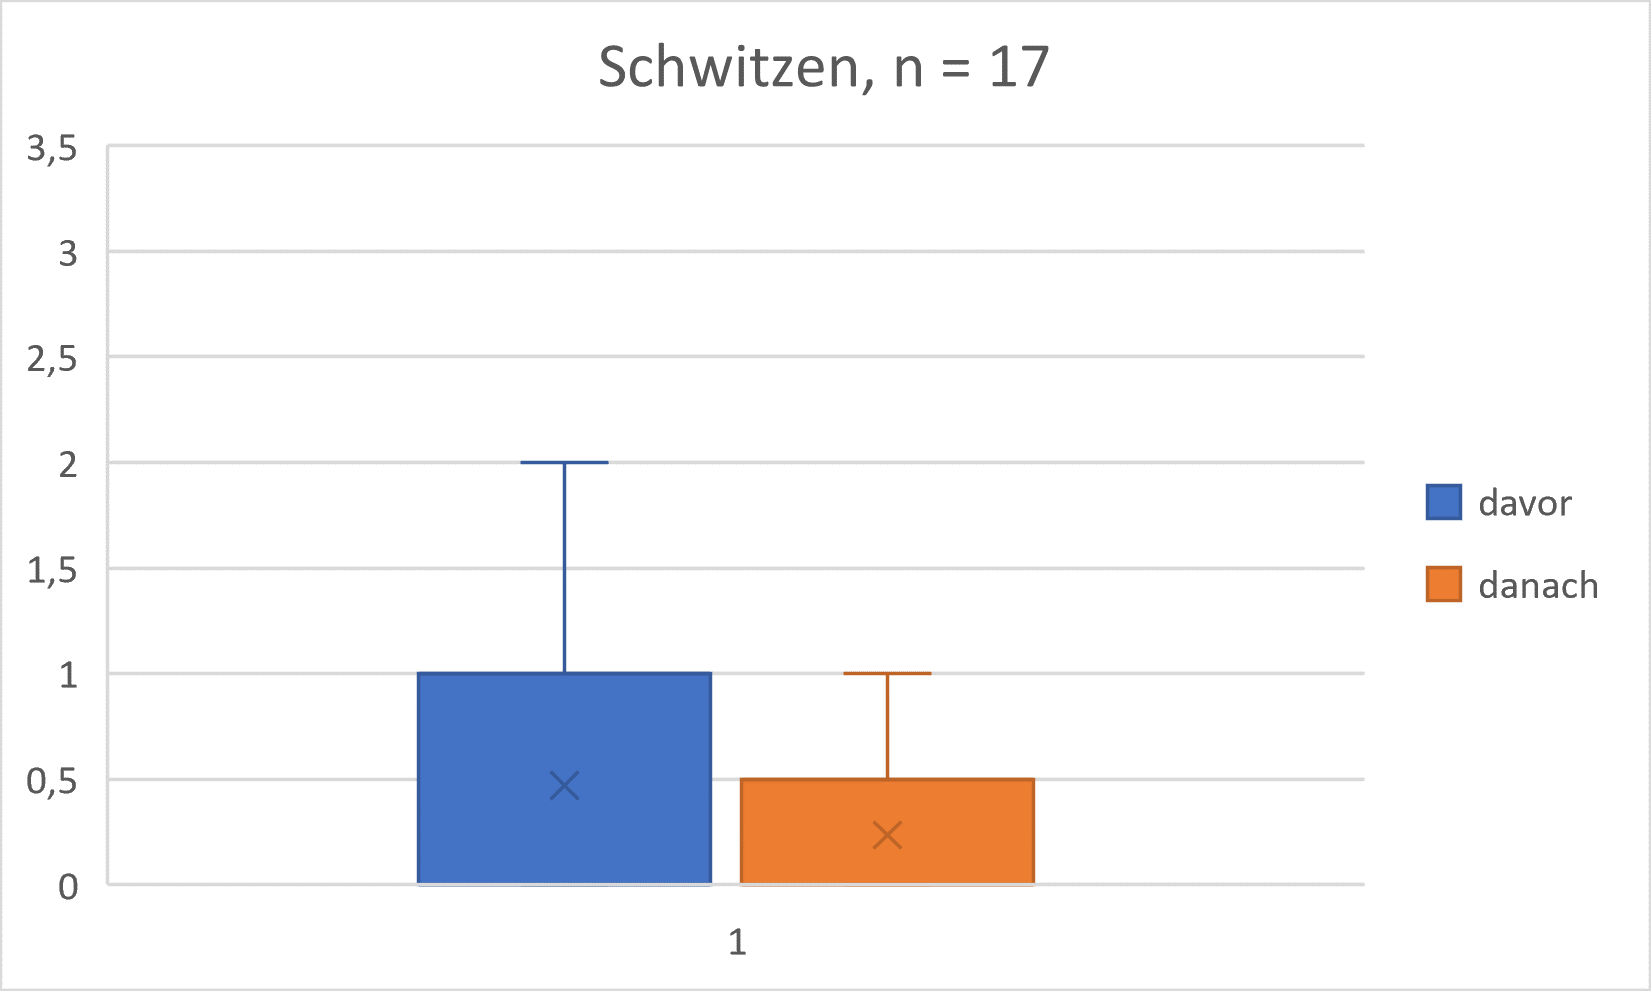
\includegraphics[width=0.2\textwidth]{assets/schwitz.png} \hspace{-5pt}
	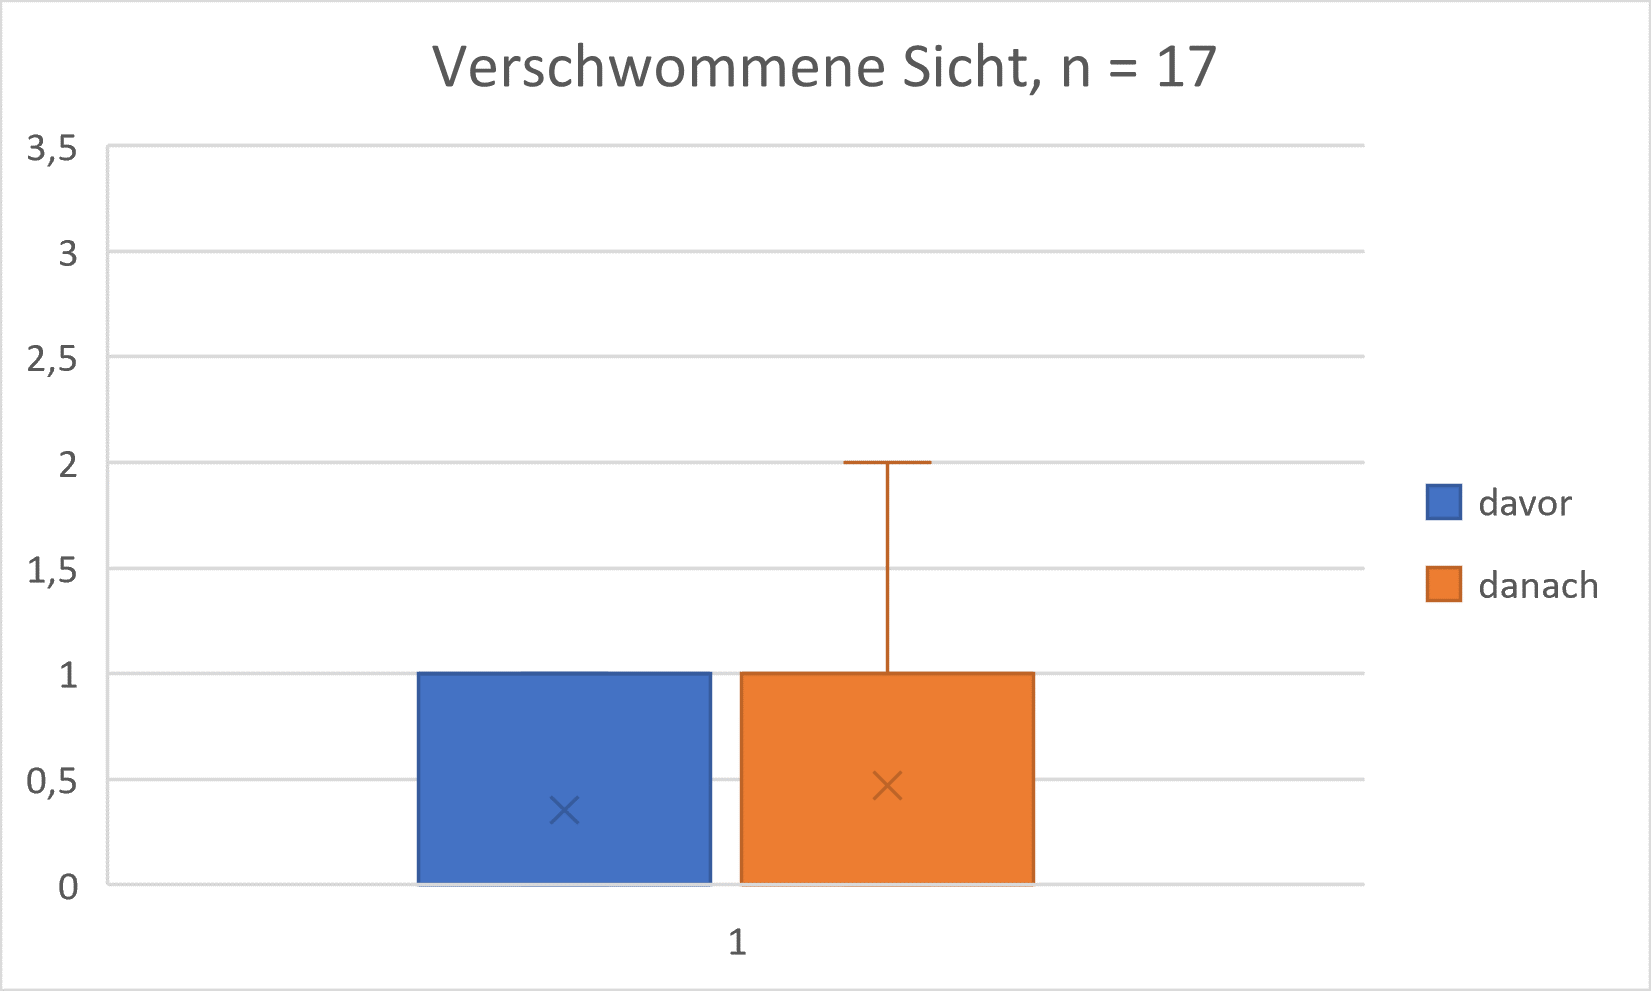
\includegraphics[width=0.2\textwidth]{assets/verschwSicht.png}
	\caption{Fragebogenergebnisse vorher nachher Vergleich}
	\label{fig:Fragebogenergebnisse}
\end{figure}

\section{Diskussion}

\section{Schlussfolgerung}

\begin{thebibliography}{00}
\bibitem{b1} J. Frey, L. Pommereau, F. Lotte und M. Hachet, 'Assessing the zone of comfort in stereoscopic displays using EEG', ACM SIGCHI Conference on Human Factors in Computing Systems (S. 2041–2046. doi: 10.1145/2559206.2581191. [Online]. Verfügbar unter: https://arxiv.org/pdf/1404.6222)

\bibitem{b2} Statista. Virtual Reality - 'Prognose zum Umsatz weltweit bis 2026' | Statista. https://de.statista.com/statistik/daten/studie/318536/umfrage/prognose-zum-umsatz-mit-virtual-reality-weltweit/ (Zugriff am: 6. Juni 2023).

\bibitem{b3} A. Tatnall, Encyclopedia of education and information technologies. SPRINGER, 2020.

\end{thebibliography}
\vspace{12pt}
\color{red}
IEEE conference templates contain guidance text for composing and formatting conference papers. Please ensure that all template text is removed from your conference paper prior to submission to the conference. Failure to remove the template text from your paper may result in your paper not being published.

\end{document}
